\documentclass{article}


% if you need to pass options to natbib, use, e.g.:
%     \PassOptionsToPackage{numbers, compress}{natbib}
% before loading neurips_2022


% ready for submission
% \usepackage{neurips_2022}


% to compile a preprint version, e.g., for submission to arXiv, add add the
% [preprint] option:
    \usepackage[preprint]{neurips_2022}


% to compile a camera-ready version, add the [final] option, e.g.:
    % \usepackage[final]{neurips_2022}


% to avoid loading the natbib package, add option nonatbib:
%    \usepackage[nonatbib]{neurips_2022}


\usepackage[utf8]{inputenc} % allow utf-8 input
\usepackage[T1]{fontenc}    % use 8-bit T1 fonts
\usepackage{hyperref}       % hyperlinks
\usepackage{url}            % simple URL typesetting
\usepackage{booktabs}       % professional-quality tables
\usepackage{amsfonts}       % blackboard math symbols
\usepackage{nicefrac}       % compact symbols for 1/2, etc.
\usepackage{microtype}      % microtypography
\usepackage{xcolor}         % colors
\usepackage{graphicx}
\usepackage{amsmath}




\title{Cheating Detection in Zero-Sum Games for Mixed Multi-Agent Environments}

\author{%
  Aishik Pyne \\
  A0250592E\\
  % \texttt{aipyne@comp.nus.edu.sg} \\
  % examples of more authors
  \And
   Harshavardhan Abichandani \\
  A0250610X\\
  % \texttt{harsh@comp.nus.edu.sg} \\
  \And
   Niharika Shrivastava\\
  % \thanks{Use footnote for providing further information
  %   about author (webpage, alternative address)---\emph{not} for acknowledging
  %   funding agencies.} \\
  A0254355A\\
  % \texttt{niharika@comp.nus.edu.sg} \\
}

\begin{document}
\maketitle

\begin{abstract} %N

Multi-agent reinforcement learning (MARL) is a prevalent learning paradigm for solving stochastic games. Specifically, imperfect information games model strategic interactions between multiple agents with only partial information which can be modelled as a POMDP \cite{pomdp:blog}. In most MARL studies, agents in a game are defined as teammates or enemies beforehand and these relationships among the agents are known to all. However, in real-world problems, the agent relationships are commonly unknown in advance. Therefore, training policies for such situations in the face of imperfect information and ambiguous identities is a significant problem that needs to be addressed. In this project, we aim to model the scenario for multi-agent partially-observable zero-sum games (e.g., poker, red-10) where $M$ agents play collaboratively against $(N-M)$ competitive agents. However, the $(N-M)$ agents unknowingly assume a fully competitive setting. With such a secret arrangement between the collaborative agents to split the reward equally after a game, we wish to observe if the collaborative agents can develop a strategy to beat the competitive agents on expectation. We also provide a discriminator that observes each agent's entire gameplay and detects cheating (a collaboration between $M$ agents).

\end{abstract}

\section{Introduction} %N

Most AI systems nowadays are based on a single agent tackling a task, or in the case of adversarial models, multiple agents compete against each other to improve the overall behaviour of a system \cite{marl:blog}. However, many real-world scenarios require a mixed setting where multiple agents act either collaboratively or competitively with each other at different timesteps to get the best returns for themselves (e.g., driving a car to reach the destination in the shortest time while avoiding traffic). In this aspect, multi-agent reinforcement learning (MARL) is a prevalent learning paradigm for solving stochastic games. Imperfect-information games model strategic interactions between multiple agents with only partial information (e.g., poker, blackjack, red-10). Typically in such games, one seeks a Nash equilibrium \cite{NashEq}, in which no player can improve by deviating from the equilibrium. Currently, the most successful algorithms for partially observable zero-sum games are Deep CFR \cite{dcfr:2018}, NFSP \cite{nsfp:2016}, and ReBel \cite{rebel:2020}. 

It is interesting to note that in most multi-agent works, whether an agent is acting collaboratively or competitively with other agents is known by everyone from the beginning which affects everyone's policies. However, in a real-life scenario, such an assumption may not always hold (e.g., a game of poker where 2 agents have teamed up against all other players with the intent of cheating). Therefore, we aim to model such a partially-observable mixed environment where individual agents attempt to maximize their reward assuming a fully competitive setting, but the teammates acting collaboratively are expected to win most games on average by maximizing their combined reward, at the expense of lower individual rewards. Such cheating scenarios are common in highly-dynamic, complex environments such as casinos. Therefore, we also train a cheating detector system that is able to observe the entire game state at all times along with the game-plays of every agent and is able to classify if there was any foul play during the game. Our contributions are as follows:

\begin{enumerate}
    \setlength{\itemsep}{0pt}
    \item We train poker agents where the policy for each agent is learned in a fully-competitive setting using NFSP \cite{nsfp:2016}.

    \item We train poker agents where two agents play collaboratively against $N$ competitive players in order to beat them in most games. Just as in a real-life case, each player's game space is still partially observable but the expected team reward is maximized.

    \item Model a discriminator that learns to distinguish between these two styles of play (competitive vs collaborative) by comparing the actions taken by each player with our trained policies. 
\end{enumerate}


\section{Related Work} %H, add NFSP

There are many approaches developed for finding nash equilibrium in games with imperfect information \cite{rebel:2020, dcfr:2018, nsfp:2016, deepstack}. We will be focusing on the two most popular approaches, Neural Fictitious Self Play and Deep Counterfactual Regret Minimization.

Neural Fictitious Self Play (NFSP) \cite{nsfp:2016} is one of the algorithms used to train agents for imperfect information games (eg. poker) which combines fictitious self play with neural networks. It is a two stage process, which can be thought of as an actor-critic framework. There is a critic which is trained using DQN. Critic stores all the $<S, A, R, S'>$ tuples in it's buffer and it is used to predict the value of the actions taken by the agent. The second part is an actor, which is trained using supervised learning. It's buffer is populated with $<S, A>$ pairs only when we sample the best response action from the critic. It learns the average policy and is used during evaluation.


% During training, the agent plays against itself. The algorithm consists of two memory buffers, first contains the experience collected from playing other agents. This memory is used to predict the value of the actions taken by the agent. Second, contains the experience of agent's own behaviour which is used to keep track of its own average behavior.

Deep Counterfactual Regret Minimization (Deep CFR) \cite{dcfr:2018}, it combines CFR with neural networks. It builds on CFR which traverses the search space and accumulates the regrets at each stage. Strategy is chosen based on algorithms which work on the principle of regret minimization. CFR cannot be used to for games with large state space, to solve this Deep CFR uses neural networks to approximate the rest of the state space. In Deep CFR at every iteration the game tree is partially traversed $K$ times and the paths are sampled using MCCFR. After the traversals, a neural network is used to predict the value of exploring that node. This can be thought of as instantaneous regrets in the CFR algorithm. 

% The above methods consider only one to one competitive play, for problems with mixed environment having $N \geq 3$ players the most popular algorithm is MADDPG \cite{maddpg}. MADDPG works by having a centralized critic that is trained using global observation and the private observation of the agents, but at test time the agents only act on the local information.

\section{Background}

\subsection{Poker Rules} %H 

Limit Texas Hold'em Poker consists of $N$ players playing for four rounds. Each player get two hand cards from a deck of $52$ shuffled cards, and at each round new community cards are revealed. In each round a player can choose between four actions (call, check, raise, fold). In Limit Texas Hold'em the number of raises is capped to four in each rounds, and the max raise amount is $1.5$x the big blind. After four rounds, the best hand wins and that player gets the total chips in the pot. Since it is a zero sum game, the sum of rewards of all the players should sum to zero. This means that there will be players with negative rewards.



\subsection{POMDP} %N

We model Poker as a Partially Observable Markov Decision Process (POMDP) which is described as the tuple $\langle S, A, T, R, O, \Omega \rangle$ where:
\begin{itemize}
    \setlength{\itemsep}{0pt}
    \item $S$ - finite set of states of the environment (game space). For Limit Texas Hold'em Poker, the game space is of the order $10^1^4$.
    
    \item $A$ - finite set of actions each agent can take at each turn (Raise, Fold, Call, Check).
    
    \item $T: S$ x $A \rightarrow \Delta(S)$ - state-transition function giving a distribution over states of the environment, given a starting state and an action performed by the agent.
    
    \item $R$ -  the reward function, giving a real-values expected immediate reward, given a starting state and an action performed by the agent. (money/chips after every game).
    
    \item $\Omega$ - finite set of observations the agent can experience.
    
    \item $O: S$ x $ A \rightarrow \Delta(\Omega)$ -  the observation function, giving a distribution over possible observations, given a starting state and an action performed by the agent.
\end{itemize}

\section{Methodology}

The section is divided into three parts. In \ref{Competitive Agent} we show how we encode the state space, evaluate and train our agents, and in \ref{Collaborative Agent} we discuss how we model the communication. Finally, \ref{Discriminator} elaborates on how we take advantage of the tractable action space to discriminate between two agents. 

\subsection{Competitive Agents} 
\label{Competitive Agent}%H
We encode the space space of limit hold'em poker into seventy two bits. The first fifty two bits contain the hand cards and the community cards. The last twenty bits contains the number of raises in each round. Limit hold'em has four rounds and each round can have a maximum of four raises. Therefore, we one hot encode this information into twenty bits. This allows us to make the state space independent of the number of players, and also includes the information about the actions taking place in the game. This way of encoding the state space is taken from the RLCard \cite{rlcard} library.

For our setting we consider a three player setting. In this setting all the agents are playing to maximize their own reward i.e. the chips they win at the end of the round. We initialize a policy network which we will refer to as "Brain 1". We first simulate a game with all the three players and generate the trajectories. Then we feed this trajectories to the neural network and train Brain 1 using the NFSP \cite{nsfp:2016} algorithm.

\subsection{Collaborative Agents} 
\label{Collaborative Agent}%H

This setting contains three agents, out of which two agents are collaborating to maximize their collective reward. To model the communication between two agents we explore two scenarios. First, the agents simply know if their friend has raised in the round. This simulates real life setting where collaborating agents need to infer from the actions. Second, we give the hand cards of the other agent along with the previous information. 

In this setting we set up rewards in the following ways.

% $$
% \mathcal{R}(s, a)= c_1 + c_2
% $$
where $c_{i}$ is the number of chips won by player $i$ after action $a$ performed in state $s$.
$$
\mathcal{R}(s, a)=\begin{cases}
			\max{c_1, c_2}, & c_3 \leq 0\\
			\displaystyle \frac{c_1 + c_2}{2}, & c_3 > 0\\
		 \end{cases}
$$
where $c_{i}$ is the number of chips won by player $i$ after action $a$ performed in state $s$.

Using the above reward function we train two agents using a policy which we will call "Brain 2". During training we are freezing the weights of the competitive agent (Brain 1) and initializing the collaborative agent with the weights of Brain 1.

\subsection{Discriminator} \label{Discriminator}%N

The action space of the game is extremely small compared to the state space ($4$ vs $10^1^4$). Therefore, we take advantage of the small action space and create a discriminator that doesn't need to enumerate the state space to detect cheating. The discriminator analyses the entire trajectory of an agent and predicts if the behaviour is closely related to Brain1 or Brain2. In Figure \ref{fig:cheating}, we see that only enumerating the actions that match with either of the Brains and not both (green and blue boxes) is sufficient to determine the behaviour of the agent on expectation over multiple games. 

\begin{figure}[h]
    \centering
    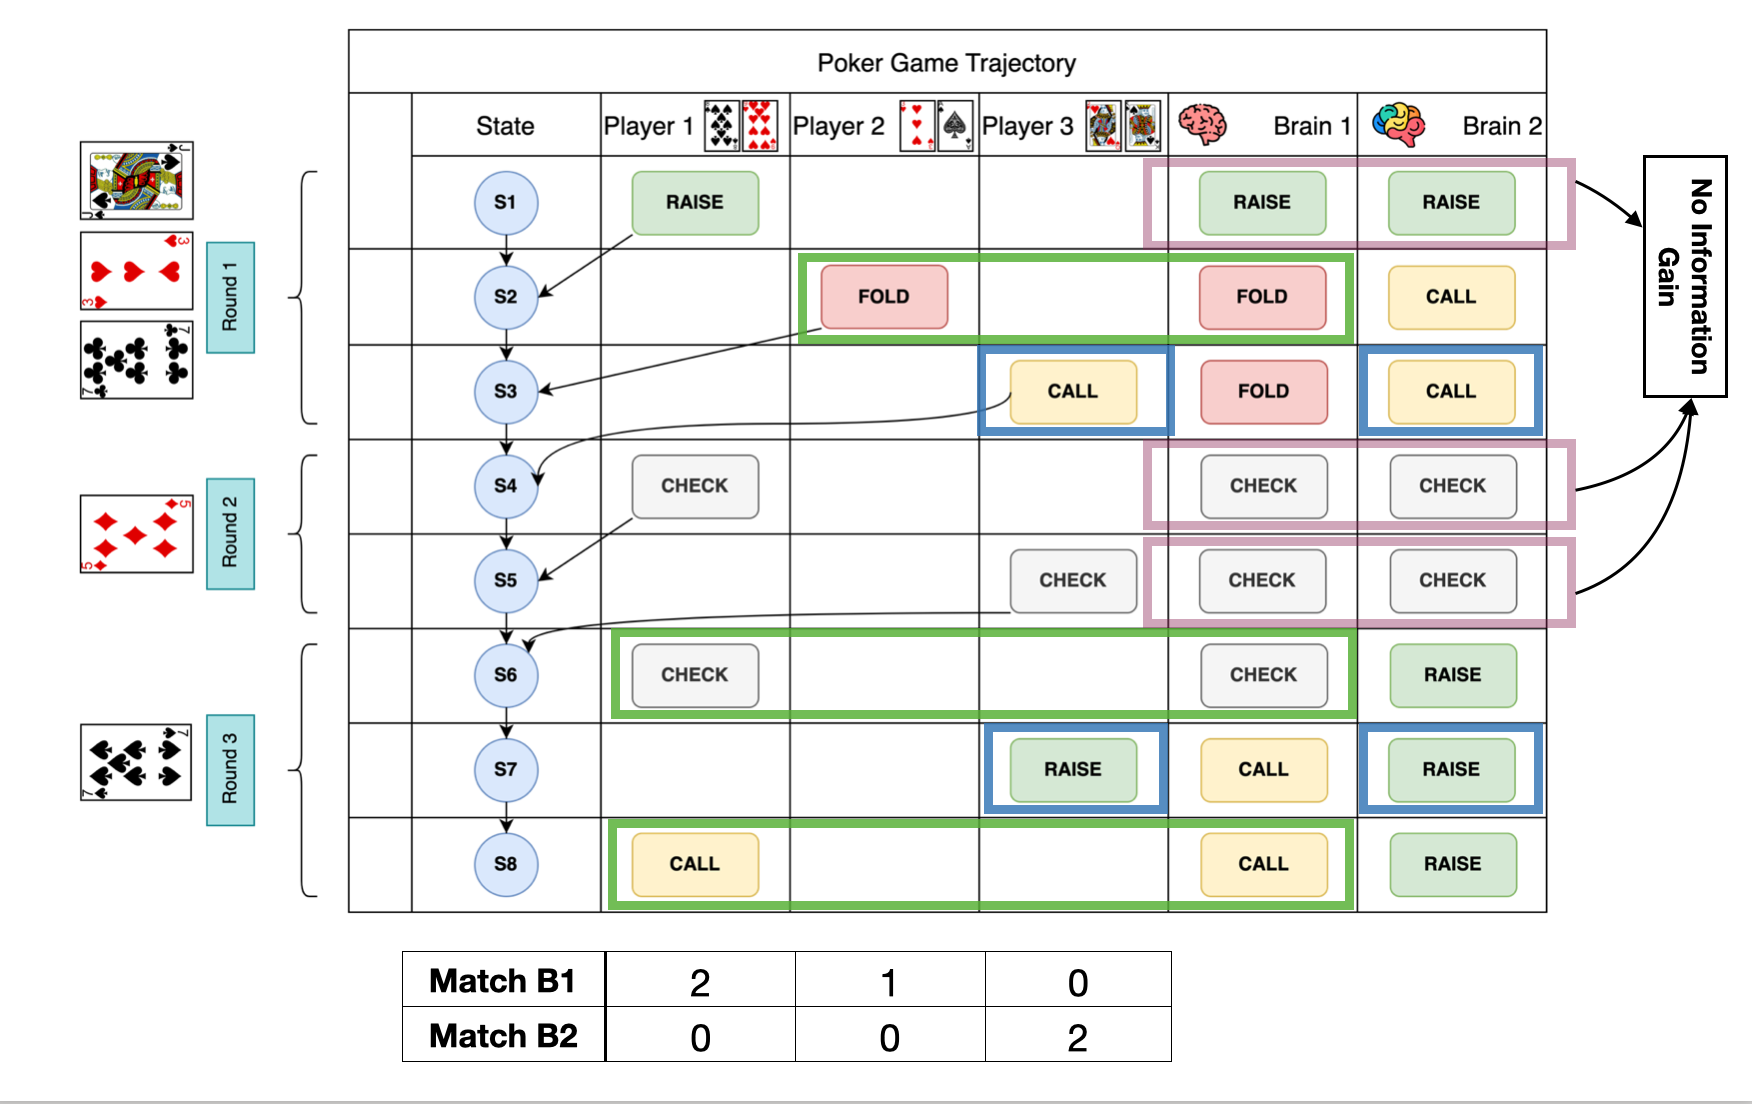
\includegraphics[width=15cm]{./images/discriminator.png}
    \caption{The pink boxes show no information gain since both the Brains exhibit the same behaviour. The green and blue boxes depict the actions of each agent that match Brain1 and Brain2 respectively. }
    \label{fig:cheating}
\end{figure}
Specifically, there is no information gain in terms of behaviour deduction if both brains choose the same action for a given state (pink boxes). However, for state spaces that provide different actions for both brains (green and blue boxes), we sum the number of times the agent matches the actions with a specific brain. Over a large number of games, the agent's true behaviour would closely imitate the behaviour of either brain. Therefore, the discriminator would be able to detect if an agent is cheating or playing fairly over an expectation.

\section{Experiments}
This section will discuss the parameters and the results of the following experiments.

\subsection{Training Results for Competitive agent} %H
We trained the three agents for $85k$ games and evaluated the agents against rule based poker agent and random agent. Brain 1 (policy network) consisted of a simple two layer mlp with $64$ neurons and was trained using the nfsp \cite{nsfp:2016} algorithm.

\begin{figure}[h]
    \centering
    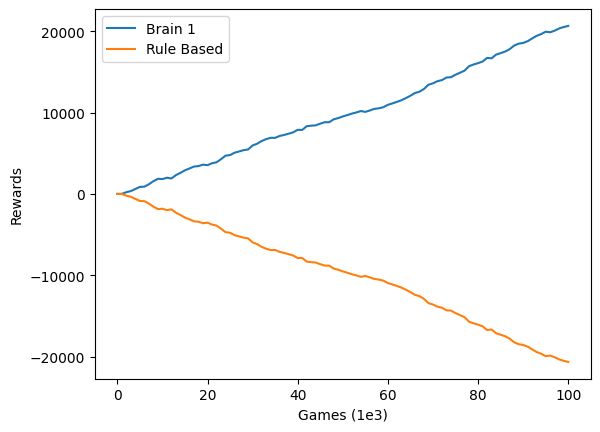
\includegraphics[width=7cm]{./images/single_rule.png}
    \caption{Brain 1 vs Rule Based agents accumulated reward over number of games.}
    \label{fig:single_rule}
\end{figure}

We compare Brain 1 with a rule based poker agent, which takes actions by calculating the probability of winning based on the hand and community cards. We do this to see if our policy is making complex strategies which do not rely on simple probabilities. Brain 1 achieves a win ratio of $3.66$ over the rule based agent, and we can see that in figure \ref{fig:single_rule} Brain 1 is accumulating more rewards over time.



Since our framework does not depend on the type of algorithm we use to train, we can confidently say that Brain 1 has at least learned some complex strategy to defeat naive poker algorithms.

\subsection{Training Results for Multi agent} %H
In this setting we kept the policy network size same, to maintain consistency. We trained the collaborative agents for $85k$ games and evaluated based on the win ratio and rewards accumulated over time. 

As we can see in Figure \ref{fig:train_4_bits_multi} that collaborative agents over time learn how to consistently defeat the competitive agent. This means that just by adding the information if the collaborative agent raised in that round, is enough to make it outperform. We also simulate $100k$ independent games and find that collaborative agents have a win ratio of $1.14$ over the competitive agent. Which means that on average it is winning $14\%$ more games.

%Add training graph of 4 bits information
\begin{figure}[h]
    \centering
    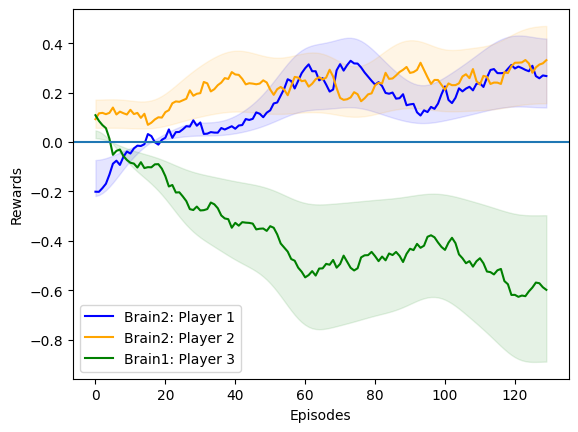
\includegraphics[width=7cm]{./images/train_4bits_multi.png}
    \caption{Training graph of collaborative setting.}
    \label{fig:train_4_bits_multi}
\end{figure}

We find out the marginal action distribution of Brain 1 vs Brain 2. Since state space is intractable, we are computing trajectories for $100k$ independent games and keeping track of the actions taken by the policies. In figure \ref{fig:confusion_matrix} we can see that Brain 2 is performing more number of raises. Which makes intuitive sense, since collaborative agents have more chances of winning, it can afford to take more risks.


\begin{figure}[h]
    \centering
    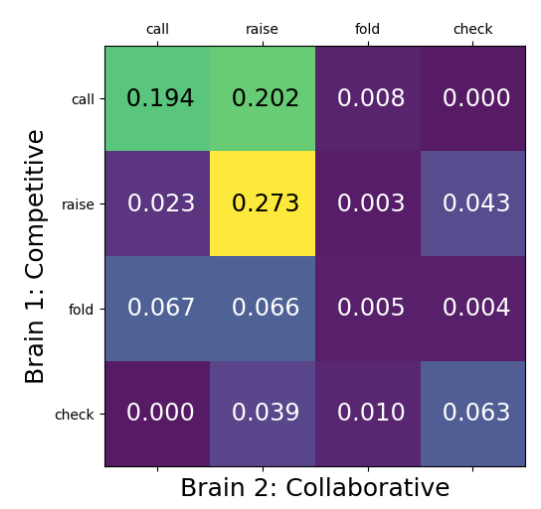
\includegraphics[width=6cm]{./images/confusion_matrix.png}
    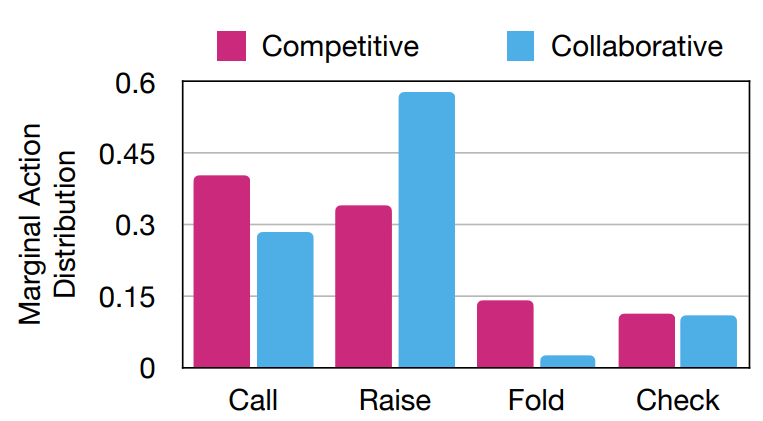
\includegraphics[width=6cm]{./images/bar_graph.png}
    \caption{Action distribution of Brain 1 vs Brain 2, $p(B_1, B_2)$}
    \label{fig:confusion_matrix}
\end{figure}


\subsection{Discriminator} %N

\begin{figure}[h]
    \centering
    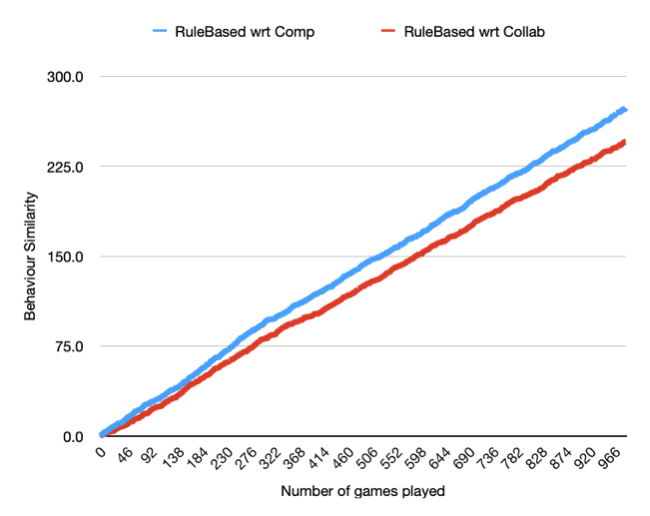
\includegraphics[width=4.5cm]{./images/rulebased.png}
    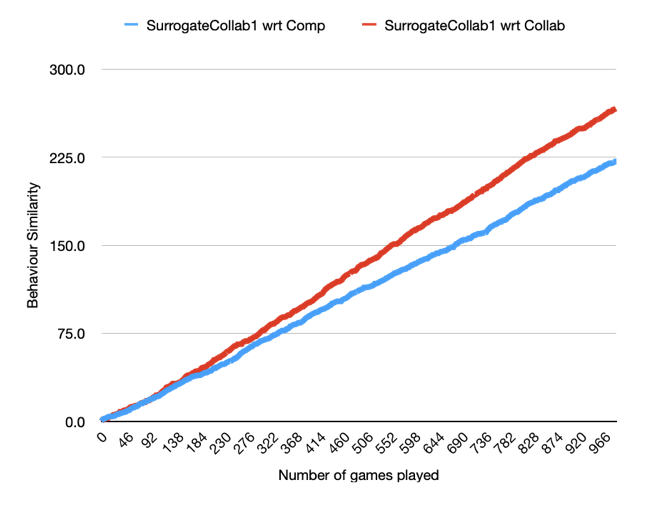
\includegraphics[width=4.5cm]{./images/cheater1.png}
    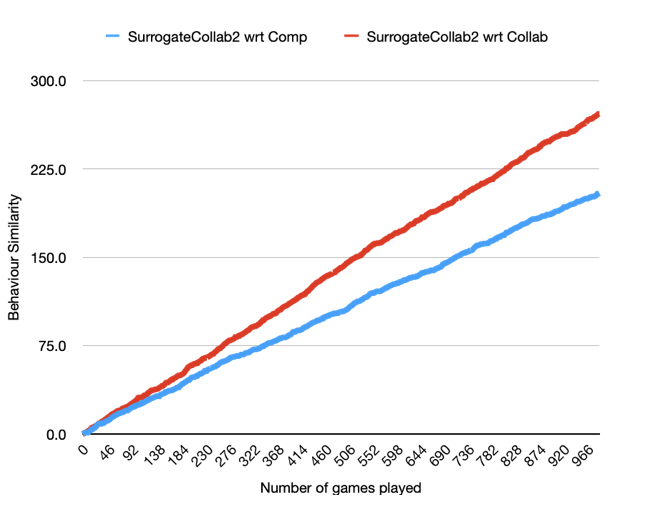
\includegraphics[width=4.5cm]{./images/cheater2.png}
    \caption{Discriminator: Similarity plots of (a) rule-based (b) collaborative teammate 1, and (c) collaborative teammate 2 agents with respect to fair and foul plays.}
    \label{fig:discriminator}
\end{figure}

The plots in Figure \ref{fig:discriminator} show that a rule-based agent is similar to a competitive (fair) player, whereas both the collaborative agents demonstrate high foul play behaviours over an increasing number of games. This is an intuitive result since a rule-based agent has no information about any other player's hand or the motivation for making any raises (bets), and plays only to maximize their own reward.

\section{Conclusion} %N

In this project, we have successfully trained multi-agents in a fully competitive and mixed environment to play a zero-sum game. We also modelled a strategy that enables the collaborative agents to win over the competitive agents on average and analysed this performance using multiple evaluation metrics. Finally, we provided an easy method to model a discriminator that can classify the behaviour of the agents as either fair or foul by analysing their individual gameplays. 

\section{Future Works \& Discussions} %H
Current evaluation and training methods are done on independent games, which makes the problem easier. So there is no long term strategy employed by the agents to win the game. We plan to train the agents on dependent games, where the winning of one game will impact the next game. Moreover, it is not intuitive that just by adding the information of which player raised makes the collaborative agent outperform the competitive agent. While there is strict information gain, it doesn't lead to any semantic meaning in real life setting.

\newpage

\bibliographystyle{plain}
\bibliography{refs}

\end{document}
